\section{Can Bus Systeme}
\label{sec:Can_Bus_Controller}

%------------Bild einfügen------------
%\begin{figure}
 % \begin{center}
  %  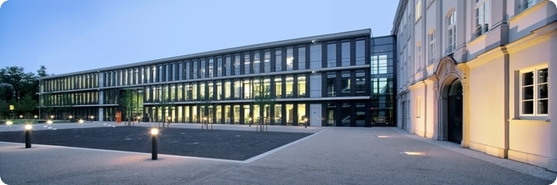
\includegraphics[width=0.6\textwidth]{./images/hochschule.jpg}
  %\end{center}
  %\vspace{-5pt}
  %\caption[Hochschule Augsburg]{Hochschule Augsburg \cite{HSA.2013}} % %Eckige Klammer (optional): Caption-Text in Abbildungsverzeichnis
  %\label{fig:hochschule}
  %\vspace{-5pt}
%\end{figure}

\subsection{Can Frame}
\label{subsec:can_bus_controller:can_frame}
 %Abbildung~\ref{fig:standort_rotes_tor_anfahrt_klm_bau} eos et accusam et justo duo dolores et ea rebum.

%\paragraph*{Beispiel}-----------Paragraph erstellen
%------------------- wrapfigure einfügen----------------------
%\begin{wrapfigure}{r}{0.45\textwidth}
 % \vspace{-20pt}
  %\begin{center}
  %  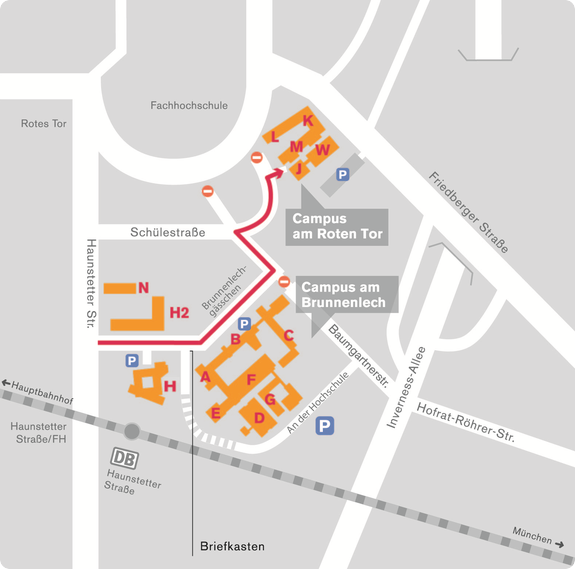
\includegraphics[width=0.45\textwidth]{./images/standort_rotes_tor_anfahrt_klm_bau.png}
  %\end{center}
  %\vspace{-20pt}
  %\caption[Standort Rotes Tor]{Standort Rotes Tor \cite{HSA.2013}}
  %\label{fig:standort_rotes_tor_anfahrt_klm_bau}
  %\vspace{-10pt}
%\end{wrapfigure}

\subsection{Can Physical Layer}
\label{subsec:can_bus_controller:can_physical_layer}



